%%%%%%%%%%%%%%%%%%%%%%%%%%%%%%%%%%%%%%%%%%%%%%%%%%%%%%%%%%%%%%%%%%% 
%                                                                 %
%                            CHAPTER                              %
%                                                                 %
%%%%%%%%%%%%%%%%%%%%%%%%%%%%%%%%%%%%%%%%%%%%%%%%%%%%%%%%%%%%%%%%%%% 
\chapter{Gebruikte data en afwijkingen}
De aanval die beschreven werd in Hoofdstuk~\ref{chap:inferentieaanval} testen
we op groep aantal gebruikers met hun desbetreffende activiteiten, om zo
zinvolle conclusies te trekken over de vatbaarheid van gebruikers op
fitnessplatformen voor deze aanval. Maar het is dan ook essentieel dat een
correcte dataset wordt gebruikt, en dat de eigenschappen die deze dataset heeft
worden beschreven. We onderzoeken eigenschappen en mogelijke afwijkingen of
onregelmatigheden opdat een gefundeerde conclusie kan worden gevormd, die
eventueel bepaalde eigenschappen van de dataset mee in rekening brengt.

Aangezien deze thesis voor een stuk verder bouwt op het onderzoek
van~\citeauthor{Dhondt}, is het
evident om verder te werken op deze
dataset~\cite{Dhondt}. Deze dataset
werd volledig zelf gescraped vanaf de officiële \ac{API} van het platform
`Strava'\footnote{\url{https://www.strava.com/}}. De scope van deze dataset is
een periode van één week, startend op 11 juli 2021 00:00 \ac{UTC}. De site werd
chronologisch afgelopen en voor alle activiteiten, met sprongen van 9000
activiteiten. Let wel dat door mogelijke vertragingen door bijvoorbeeld het
uploaden van een activiteit, de activiteiten niet exact chronologisch kunnen
worden opgehaald. Indien een activiteit privaat is of gecloaked\footnote{Een
    gecloakede activiteit is een activiteit waar al een EPZ op is aangebracht.
    Aangezien deze thesis uncloaked activities nodig heeft~\ref{sec:zelf_cloaking}
    zijn ze dus niet bruikbaar. Men kan zien of een activiteit gecloaked is indien
    er een verschil is tussen de zichtbare afstand en de totale afstand.} is, of
reeds verwijdert is, dan zal deze worden overgeslagen en de volgende worden
genomen. Voor elke activiteit die succesvol werd gevonden, wordt daarna de
gebruiker beschouwd. Van alle bekomen gebruikers worden dan de rest van de
activiteiten afgehaald en bijgehouden in één grote dataset. De gegevens worden
ook geanonimiseerd opgeslagen, zodat de gebruikers niet meer kunnen worden
geïdentificeerd. De dataset bevat dus geen namen of andere persoonlijke
gegevens, enkel ID's.

In totaal werd een dataset van 4000 gebruikers verzameld. Deze thesis
experimenteert echter slechts met een subset van 131 users, waarvan er 101
gebruikt worden voor analyses en conclusies, en 30 voor het testen van de
aanval.

\section{Karakteristieken van de gebruikte dataset}
Op Figuur~\ref{fig:geographic_spread} is de geografische spreiding van de
activiteiten gevisualiseerd aan de hand van een heatmap. Hierop is duidelijk te
zien dat de meeste activiteiten zich in Centraal-Europa bevinden. Daarnaast is
ook een duidelijke concentratie te zien in de Verenigde Staten. In mindere mate
zijn ook activiteiten in Australië en Zuid-Amerika. De dataset bevat dus
relatief een grote spreiding van activiteiten over de hele wereld, wat een
goede basis is voor het testen van de aanval. Let wel, de dataset is met 101
gebruikers echter wel relatief klein, wat een vertekend beeld kan geven van de
werkelijkheid.

Op Tabel~\ref{tab:stats_dataset} zijn enkele globale statistieken met
betrekking tot gebruikers en de bijhorende activiteiten van de dataset
weergegeven. Er valt op dat de dataset per gebruiker toch meestal een groot
aantal activiteiten ter beschikking zijn. De gemiddelde gebruiker bevat 411
activiteiten, de mediaan is 296. Volgens de inferentieaanval beschreven in
Hoofdstuk~\ref{chap:inferentieaanval} resulteert een gebruiker met meer
activiteiten over het algemeen in een accuratere aanval. Op
Figuur~\ref{fig:cdf_amount_activities} is de \ac{CDF} plot\footnote{Een
    Cumulative Distribution Function (CDF) plot is een grafiek die de cumulatieve
    verdeling van de waarden van een continue variabele
    weergeeft~\cite{CursusSt38:online}. De x-as van de grafiek bevat de
    verschillende waarden die de continue variabele kan aannemen, terwijl de y-as
    de kans aangeeft dat de variabele een waarde kleiner dan of gelijk aan die op
    de x-as aanneemt. De curve van de CDF laat zien hoe waarschijnlijk het is dat
    een willekeurige waarde van de continue variabele kleiner is dan een bepaalde
    drempelwaarde.} te zien die het aantal activiteiten per gebruiker weergeeft.
Hierop worden voorgaande besluiten enkel maar bevestigd. Het plot duidt ook aan
dat meer dan 20\% van de gebruikers een aantal activiteiten heeft dat groter is
dan 100.

\begin{figure}[h]
    \centering
    \includegraphics[width=\textwidth]{fig/Afwijkingen&Analyses/Heatmap.png}
    \caption{Geografische spreiding van de activiteiten in de dataset}\label{fig:geographic_spread}
\end{figure}
\begin{table}[h]
    \centering
    \begin{tabular}{|l||c|}
        \hline
        \textbf{Waarde}                       & \textbf{Aantal} \\
        \hline \hline
        Total number of users                 & 101             \\
        \hline
        Total number of activities            & 41 554          \\
        \hline
        Average \# activiteiten per user      & 411             \\
        \hline
        Median of \# activities per user      & 296             \\
        \hline
        Maximal \# activities for single user & 2946            \\
        \hline
        Minimal \# activities for single user & 31              \\
        \hline
    \end{tabular}
    \captionsetup{justification=centering}
    \caption{Overzicht van gebruikers en activiteiten}\label{tab:stats_dataset}
\end{table}
\begin{figure}[h]
    \centering
    \includegraphics[width=0.9\textwidth]{fig/Afwijkingen&Analyses/CDF_amountActivities.jpg}
    \caption{\ac{CDF} plot van het aantal activiteiten per gebruiker}\label{fig:cdf_amount_activities}
\end{figure}

Let wel, alhoewel niet expliciet vermeld
door~\citeauthor{Dhondt}, is er een
vermoeden dat er bewust gezocht werd naar gebruikers met een zo groot mogelijk
aantal activiteiten per gebruiker. Dit is een logische keuze, aangezien de
aanval een hogere kans op slagen heeft bij users die meer activiteiten hebben.
Wanneer we dit vergelijken met cijfers uit een studie die Strava zelf voerde in
2020, is er toch een mismatch terug te vinden~\cite{StravaMi72:online}. Het
persbericht, waarvan Figuur~\ref{fig:3billionUsers} is overgenomen, stelt dat
Strava in 2020 iets meer dan 50 miljoen gebruikers had, die samen in totaal
drie miljard activiteiten op het platform hebben geplaatst. Indien we deze
waarden omrekenen naar een gemiddelde, komen we uit op een ruwe geschatte 60
activiteiten per gebruiker ($\frac{3 \cdot 10^9}{5 \cdot 10^7} = 60 $). Dit is
een stuk lager dan de gemiddelde 411 activiteiten per gebruiker in de dataset.
De conclusies die dus getrokken worden uit deze steekproef mogen niet zomaar
veralgemeend worden naar de volledige gebruikersbasis van Strava.
\begin{figure}[H]
    \centering
    \includegraphics[width=0.5\textwidth]{fig/Strava_3billion.png}
    \caption{Post op sociale media van Strava die de evolutie van het totaal aantal activiteiten weergeeft~\cite{StravaMi72:online}}\label{fig:3billionUsers}
\end{figure}

\section{Mogelijke afwijkingen binnenin de dataset}
Doordat de dataset niet expliciet werd gecheckt op onnauwkeurigheden en een
willekeurige sample is, Doordat deze dataset niet door Strava zelf werd
vrijgegeven, maar manueel afgehaald werd via scraping, is er een grote kans op
activiteiten die afwijkingen of fouten vertonen. Zeker door het belang van
\ac{gps}-data, die een grote kans heeft op fouten, in deze studie is het
belangrijk om de dataset te analyseren op deze mogelijke afwijkingen. Gps-data
is een signaal die a.d.h.v.\ gekende locaties van satellieten, gecombineerd met
de tijd die het signaal nodig heeft om deze satellieten te bereiken, de locatie
van een gebruiker kan bepalen~\cite{BadGPSDa19:online}. Door de snelheid van
het signaal, kunnen kleine vertragingen in het signaal al een grote invloed
hebben op de accuraatheid van de data. Andere factoren zoals hoge bomen of
gebouwen, maar ook de aanwezigheid van wolken kunnen een impact hebben op het
signaal. Ook de frequentie waarmee locatie wordt bepaald, wat afhankelijk is
van het gebruikte toestel kan meespellen.

\subsection{Mogelijke fouten bij gps-data}
Zoals reeds aangehaald kunnen er bij het verzamelen van \ac{gps}-data
significante fouten optreden. Met \ac{gps}-fouten wordt gedoeld op data die de
\ac{gps}-sensor opvangt die niet overeenstemt met de werkelijke
\ac{gps}-locatie. Deze fouten kunnen verschillende oorzaken hebben. De
belangrijkste zijn hierbij \textit{\ac{gps}-drift}, \textit{\ac{gps}-signal
    loss} en \textit{\ac{gps}-bounce}.

Gps-drift is een fenomeen waarbij de \ac{gps}-locatie van een gebruiker afwijkt
van de effectieve locatie. Een voorbeeld vanuit het Strava-platform is terug te
vinden op Figuur~\ref{fig:gps_drift_Strava}. Hierbij is te zien dat de
gebruiker een deel van de route door gebouwen heen en door het water aflegt.
Dit kan worden veroorzaakt door dichtbebouwde omgevingen, en omgevingsfactoren
zoals hoge bomen. Om dit tegen te gaan, zou eventueel de eerder beschreven
methode van map-snapping kunnen worden toegepast.
\begin{figure}[h]
    \centering
    \begin{subfigure}[b]{.45\textwidth}
        \centering
        \includegraphics[width=\textwidth]{fig/Afwijkingen&Analyses/Crooked Routes/GPS-drift.png}
        \caption{Voorbeeld van gps-drift op Strava}\label{fig:gps_drift_Strava}
    \end{subfigure}\hfill
    \begin{subfigure}[b]{.49\textwidth}
        \centering
        \includegraphics[width=\textwidth]{fig/Afwijkingen&Analyses/Crooked Routes/GPS-Drift_onlnie.jpg}
        \caption{Voorbeeld van gps-drift op een satellietkaart, veroorzaakt door dichte boomgroei~\cite{BadGPSDa19:online}}
    \end{subfigure}
    \caption{Voorbeelden van gps-drift}
\end{figure}

Gps-bouncing is een fenomeen veroorzaakt door hoge gebouwen. Het
\ac{gps}-signaal zal hierbij over en weer weerkaatsen tussen de gebouwen, op
weg naar de satelliet. Hierdoor verondersteld het apparaat afgelegde afstand
bij het berekenen van de locatie, door de extra vertraging. De uitkomst van het
traject is dan onvoorspelbaar, wat leidt tot een `cluster' van \ac{gps}-punten
wanneer dit voor een paar punten in dezelfde omgeving gebeurt. Voorbeelden
hiervan zijn terug te vinden op Figuur~\ref{fig:gps_bounce}. Om dit fenomeen op
zijn beurt tegen te gaan, is het best om smoothing te toe te passen bij het
berekenen.
\begin{figure}
    \centering
    \begin{subfigure}[b]{0.49\textwidth}
        \centering
        \includegraphics[width=\textwidth]{fig/Afwijkingen&Analyses/Crooked Routes/Crooked GPS Route_Cart.png}
    \end{subfigure}
    \begin{subfigure}[b]{0.49\textwidth}
        \centering
        \includegraphics[width=\textwidth]{fig/Afwijkingen&Analyses/Crooked Routes/GPS_bounce_map.jpg}
    \end{subfigure}
    \caption{Voorbeelden van \ac{gps}-bounce~\cite{BadGPSDa19:online}}\label{fig:gps_bounce}
\end{figure}

Er zijn ook voorbeelden waarbij beide fenomenen voorkomen, zoals te zien is op
Figuur~\ref{fig:gps_drift_bounce_Strava}. Zoals te zien is op deze figuur, zal
indien op een intuïtieve manier de afstand wordt berekend (door gewoon het
afstandsverschil tussen twee opeenvolgende punten te nemen), een significant
verschil zijn tussen de afstand die de gebruiker werkelijk afgelegd heeft, en
de berekende afstand.
\begin{figure}
    \centering
    \includegraphics[width=0.7\textwidth]{fig/Afwijkingen&Analyses/Crooked Routes/1_notSnapped.png}
    \caption{Voorbeeld van zowel gps-drift en gps-bounce uit de gebruikte dataset}\label{fig:gps_drift_bounce_Strava}
\end{figure}

Een laatste fenomeen dat kan optreden is \ac{gps}-signal loss. Hierbij gaat het
signaal van de gebruiker verloren, en wordt pas op een later tijdstip terug een
nieuw signaal verzonden, waardoor een sprong werd gemaakt. In dit geval zou map
matching opnieuw een goede oplossing om dit te omzeilen. Een tweede oorzaak die
kan leiden tot signal loss, die zeker van toepassing is bij fitness trackers,
is de mogelijkheid tot het pauzeren van een activiteit. In dit geval wordt de
activiteit gepauzeerd voor een bepaald tijdsframe, en wordt er geen data meer
verzameld. Wanneer de activiteit terug wordt hervat, zal er een sprong zijn in
de \ac{gps}-locaties, wat kan leiden tot een verkeerde berekening van de
afstand. In het geval van een pauze zal mapmatching geen oplossing zijn, maar
zou deze `sprongafstand' best weggelaten worden in de berekeningen. Een
voorbeeld hiervan is terug te vinden op Figuur~\ref{fig:gps_signal_loss}.
\begin{figure}
    \begin{subfigure}[b]{0.49\textwidth}
        \centering
        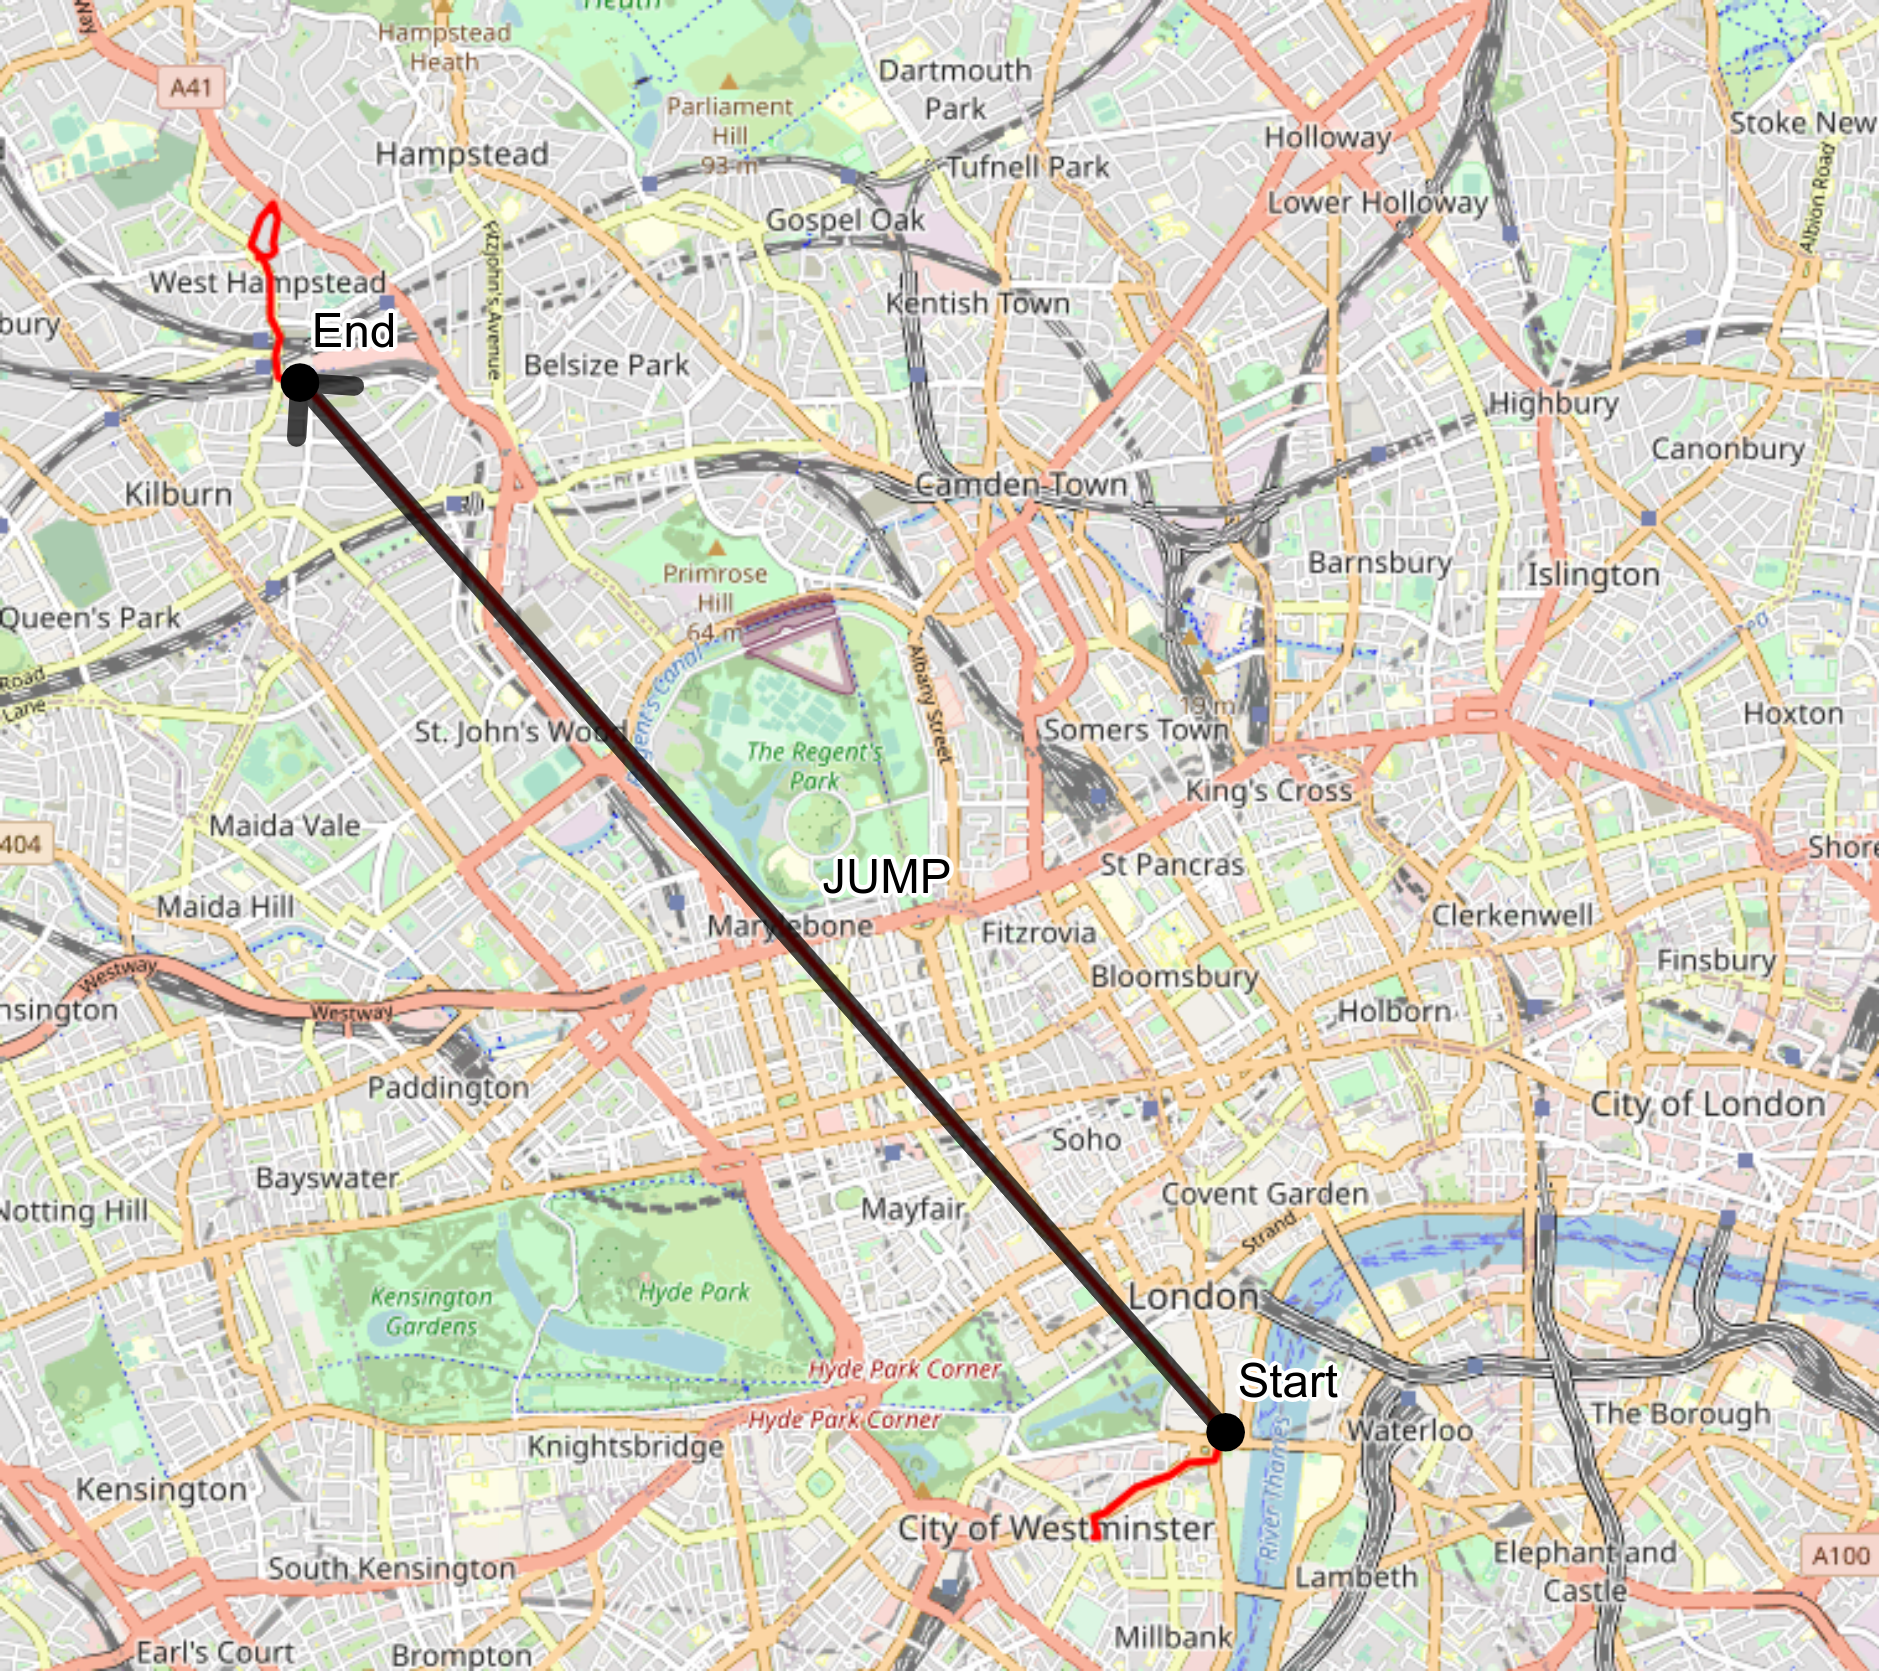
\includegraphics[width=\textwidth]{fig/Afwijkingen&Analyses/Crooked Routes/1_Full_withArrow.png}
    \end{subfigure}
    \begin{subfigure}[b]{0.49\textwidth}
        \centering
        \includegraphics[width=\textwidth]{fig/Afwijkingen&Analyses/Crooked Routes/1_Full_original.png}
    \end{subfigure}
    \caption{Voorbeeld van signal loss uit de gebruikte dataset}\label{fig:gps_signal_loss}
\end{figure}

\subsection{Gps-fouten in de gebruikte dataset}
Allereerst onderzoeken we naar de aanwezigheid van \ac{gps}-fouten in de vorm
van signal losses of pauzes. Dit gebeurt door de afstand tussen twee
opeenvolgende \ac{gps}-punten te bestuderen.
Tabel~\ref{tab:distance_between_gps_points_table} geeft een globaal overzicht
van deze verdeling, en de volledige verdeling is terug te vinden op
Figuur~\ref{fig:distance_between_gps_points_CDF}. De gemiddelde afstand tussen
twee opeenvolgende locaties is $6.41m$, met een standaardafwijking van
$42.53m$. Het gemiddelde is relatief laag, wat kan wijzen op accurate gegevens,
maar de hoge standaardafwijking wijst op grote schommelingen. Op de grafiek en
de tabel is te zien dat de meeste afstanden onder de $20m$ liggen, wat opnieuw
een indicatie kan zijn van een degelijke precisie. Er is echter wel een klein
deel van de \ac{gps}-punten die een grote onderlinge afstanden vertoond. Door
de omvang van het aantal \ac{gps}-punten, en een gemiddeld aantal punten per
activiteit van $2574.90$, valt dit zeker niet te verwaarlozen. Als we empirisch
stellen dat een significant verschil $50m$ bedraagt, dan ligt 0.9\% van de data
boven deze drempel. Per activiteit zou dit dan resulteren op gemiddeld $23$
afwijkende punten, wat zeker kan zorgen voor een significante afwijking op de
resulterende afstand.
\begin{table}[h]
    \centering
    \begin{tabular}{lr}
        \toprule
        \midrule
        Total number of gps-points              & $1.070 \cdot 10^8$        \\
        \hline
        distance between 2 gps points $>$ 10m   & $13.91\%$                 \\
        distance between 2 gps points $>$ 20m   & $5.44\%$                  \\
        distance between 2 gps points $>$ 50m   & $9.02 \cdot 10^{-1}\%$    \\
        distance between 2 gps points $>$ 75m   & $2.21 \cdot 10^{-2}\%$    \\
        distance between 2 gps points $>$ 100m  & $1.30 \cdot 10^{-2}\%$    \\
        distance between 2 gps points $>$ 150m  & $8.04 \cdot 10^{-3}\%$    \\
        distance between 2 gps points $>$ 200m  & $6.071 \cdot  10^{-3} \%$ \\
        distance between 2 gps points $>$ 500m  & $2.600 \cdot 10^{-3} \%$  \\
        distance between 2 gps points $>$ 1000m & $1.345 \cdot 10^{-3}$ \%  \\
        distance between 2 gps points $>$ 2000m & $4.056 \cdot 10^{-4} \%$  \\
        \midrule
        \bottomrule
    \end{tabular}
    \captionsetup{justification=centering}
    \caption{Verdeling van de afstanden tussen twee opeenvolgende gps-punten}\label{tab:distance_between_gps_points_table}
\end{table}
\begin{figure}
    \centering
    \includegraphics[width=\textwidth]{fig/Afwijkingen&Analyses/Graphs/Afstand tussen 2 gps-punten.png}
    \caption{Verdeling van de afstanden tussen twee opeenvolgende gps-punten}\label{fig:distance_between_gps_points_CDF}
\end{figure}

Om het aantal \ac{gps}-afwijkingen in de dataset te bepalen die relevant zijn
voor de aanval, wordt ook het verschil onderzocht tussen de berekende afstand
afgelegd buiten de \ac{EPZ} (het zichtbare traject) en de theoretisch afgelegde
afstand buiten de \ac{EPZ}, die af te lezen valt uit de dataset via de
cumulatieve afstand\footnote{Er wordt gesproken van een theoretische waarde,
    maar deze is eigenlijk de berekende waarde volgens het platform. We beschouwen
    deze dus als referentie.}. Een eerste visualisatie is te zien op
Figuur~\ref{fig:difference_noCDF}. De figuur illustreert de schommelingen
tussen de handmatig berekende afstand en de theoretische afstand van één
gebruiker. De pieken duiden op duidelijk sterk afwijkende berekende afstanden,
en dus ook op grote \ac{gps}-fouten. Maar ook de schommelingen die iets minder
opvallend zijn duiden op grote inaccuraatheden tussen de berekende en
theoretische afstanden. Voor de volledige dataset wordt gebruik gemaakt van
\ac{CDF}-plots. De resultaten worden weergegeven op
Figuur~\ref{fig:differences_theoretical}. Figuur~\ref{fig:differences_log}
bevat de verdeling voor alle activiteiten, gebruik makend van een logaritmische
schaal. Figuur~\ref{fig:differences_nolog} toont 95\% van de activiteiten met
de kleinste verschillen, om een beter beeld te krijgen van de grootte van de
meeste verschillen. Op de grafieken valt op dat heel wat significante
verschillen aanwezig zijn. Dit duidt op het relatief zwaar doorwegen van de
\ac{gps}-fouten in de dataset. Aangezien het gaat over bepalen van woonplaatsen
of andere gevoelige locaties, kunnen afwijkingen vanaf 50 à 100 meter al
relevant zijn. Daarnaast gaat het vaak over kleine afwijkingen op een heel wat
punten, wat kan resulteren in een grote afwijking. De grafieken tonen aan dat
er bij de ruwe ontvangen data heel wat \ac{gps}-fouten aanwezig zijn. Smoothing
zal dus zeker nodig zijn om deze te beperken.

\begin{figure}
    \centering
    \includegraphics[width=\textwidth]{fig/Afwijkingen&Analyses/Graphs/Verschil_Theoretische_innerDistance.png}
    \caption{Verschil tussen de berekende afstand en de theoretische afstand voor één gebruiker}\label{fig:difference_noCDF}
\end{figure}
\begin{figure}[h]
    \centering
    \begin{subfigure}{\textwidth}
        \includegraphics[width=\textwidth]{fig/Afwijkingen&Analyses/Graphs/100_Differences_tov_theoretische_BefSmoothening.png}
        \caption{100\% van de activiteiten (logaritmische schaal)}\label{fig:differences_log}
    \end{subfigure}
    \begin{subfigure}[b]{\textwidth}
        \includegraphics[width=\textwidth]{fig/Afwijkingen&Analyses/Graphs/95_Differences_tov_theoretische_BefSmoothening.png}
        \caption{95\% van de activiteiten}\label{fig:differences_nolog}
    \end{subfigure}
    \caption{Verdeling van het verschil tussen de berekende afstand en de theoretische afstand buiten de \ac{EPZ} }\label{fig:differences_theoretical}
\end{figure}

\section{Technieken gps-data te verbeteren}
Om de accuraatheid van de \ac{gps}-data te verbeteren, en zo een betere
\textit{outer distance} te kunnen berekenen en uiteindelijk een accuratere
aanval te bekomen, worden enkele technieken toegepast. Zoals besproken in
Sectie~\ref{sec:afstandsberekeningen_strava} is de hypothese dat de
fitness-platformen gebruik maken van technieken om de \ac{gps}-data te
verbeteren. De besproken technieken waren \textit{map matching} en
\textit{\ac{gps}-smoothing}. Bij de uitvoering van de aanvallen wordt smoothing
toegepast. Er wordt dan ook geëxperimenteerd met verschillende smoothing
windows, op zoek naar het window met het beste effect op de aanval.

Daarnaast passen we ook een filtering toe die rekening houdt met
\ac{gps}-sprongen. Het idee is te stellen dat wanneer \ac{gps}-sprongen
gebeuren, en er dus een te grote afstand tussen twee opeenvolgende punten is
deze afstand niet te laten meetellen. Dit is echter wel niet vanzelfsprekend,
aangezien dit wel kan worden meegenomen door de berekeningen van de platformen.
Stel dat wij een sprong van $50m$ laten vallen, maar de platformen laten deze
wel meetellen, dan zullen we de afwijking op het eindresultaat enkel maar
verhogen. Het drempel voor de filtering moet dus hoog genoeg zijn om deze
voorvallen te vermijden. In dit onderzoek kozen we voor een drempelwaarde van
$200m$.

% EXTRAAAA
% \section{Stilstaande gebruiker}
% In Sectie~\ref{sec:definitie-aanvaller} wordt de aanvaller assumptie gemaakt
% dat een gebruiker niet mag stilstaan binnen de~\ac{EPZ}. Deze is enkel van
% toepassing indien de berekening gebeurt op basis van de totale verstreken tijd. Op Figuur~\ref{fig:time_diff} zien we dat de verschillen